\subsection{Red McDonald's}

Para el siguiente experimento, capturamos los paquetes de la LAN Wi-Fi pública del McDonald's ubicado en el shopping Alto Avellaneda. La medición fue realizada un día sábado desde las 18 hs hasta las 20 hs. La cantidad de paquetes capturados es de aproximadamente 65.000. De todos estos, sólo 918 corresponden al protocolo ARP.

\begin{figure}[H]
       \centering
       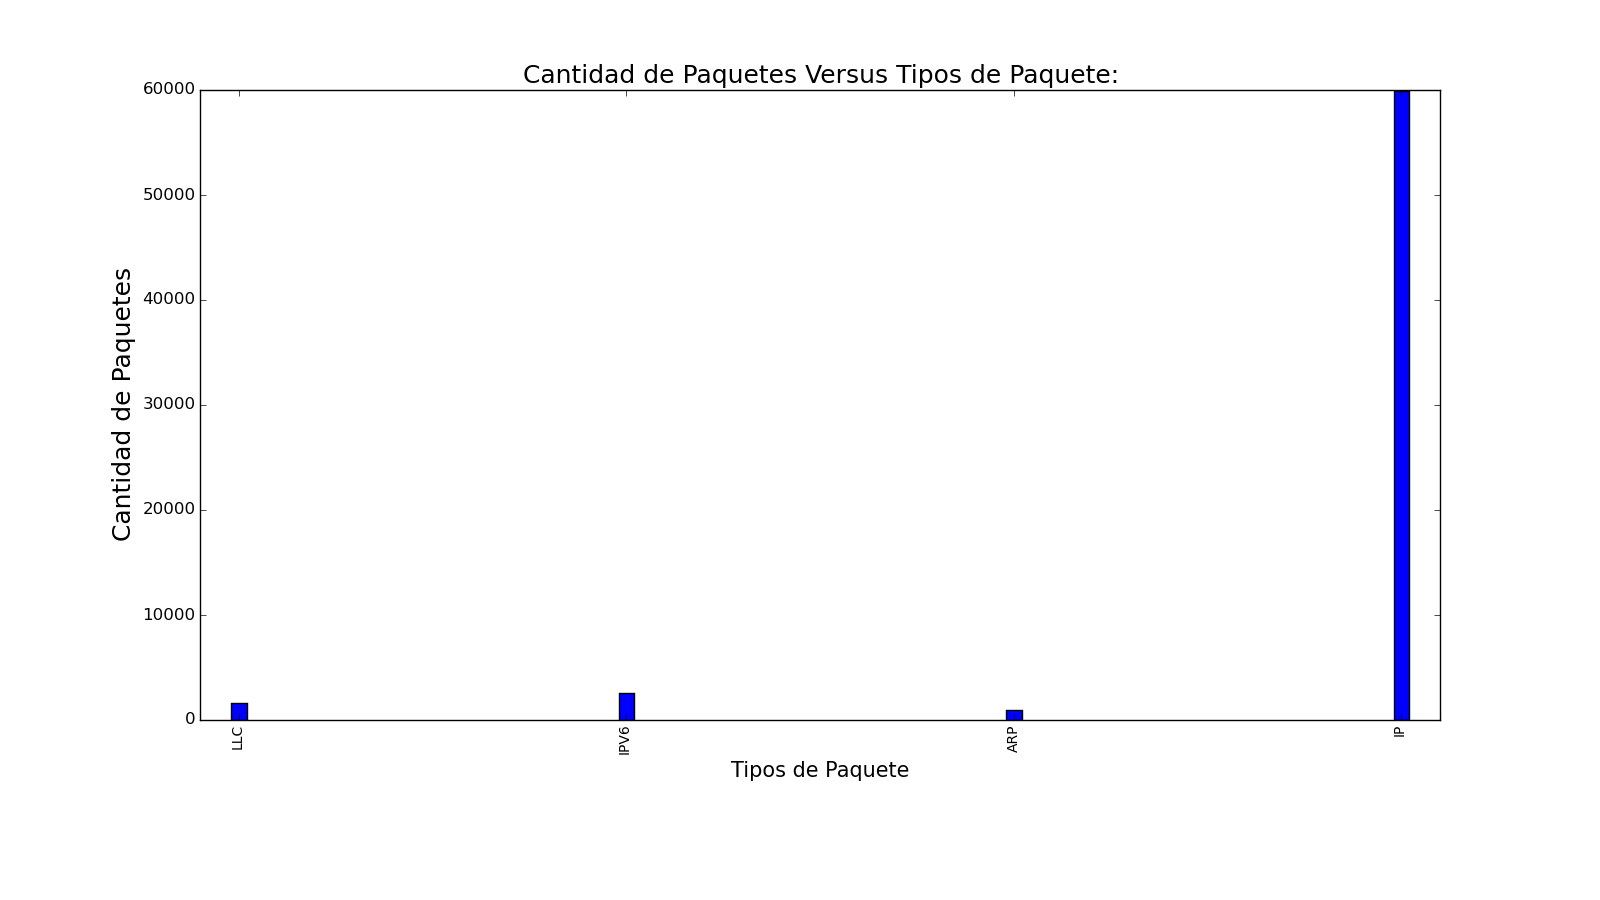
\includegraphics[width=1\textwidth]{../resultados/McDonalds/histogram_types.png}
       \caption{Protocolos de los paquetes capturados}
       \label{red-hogarena-types}
\end{figure}

\begin{figure}[H]
       \centering
       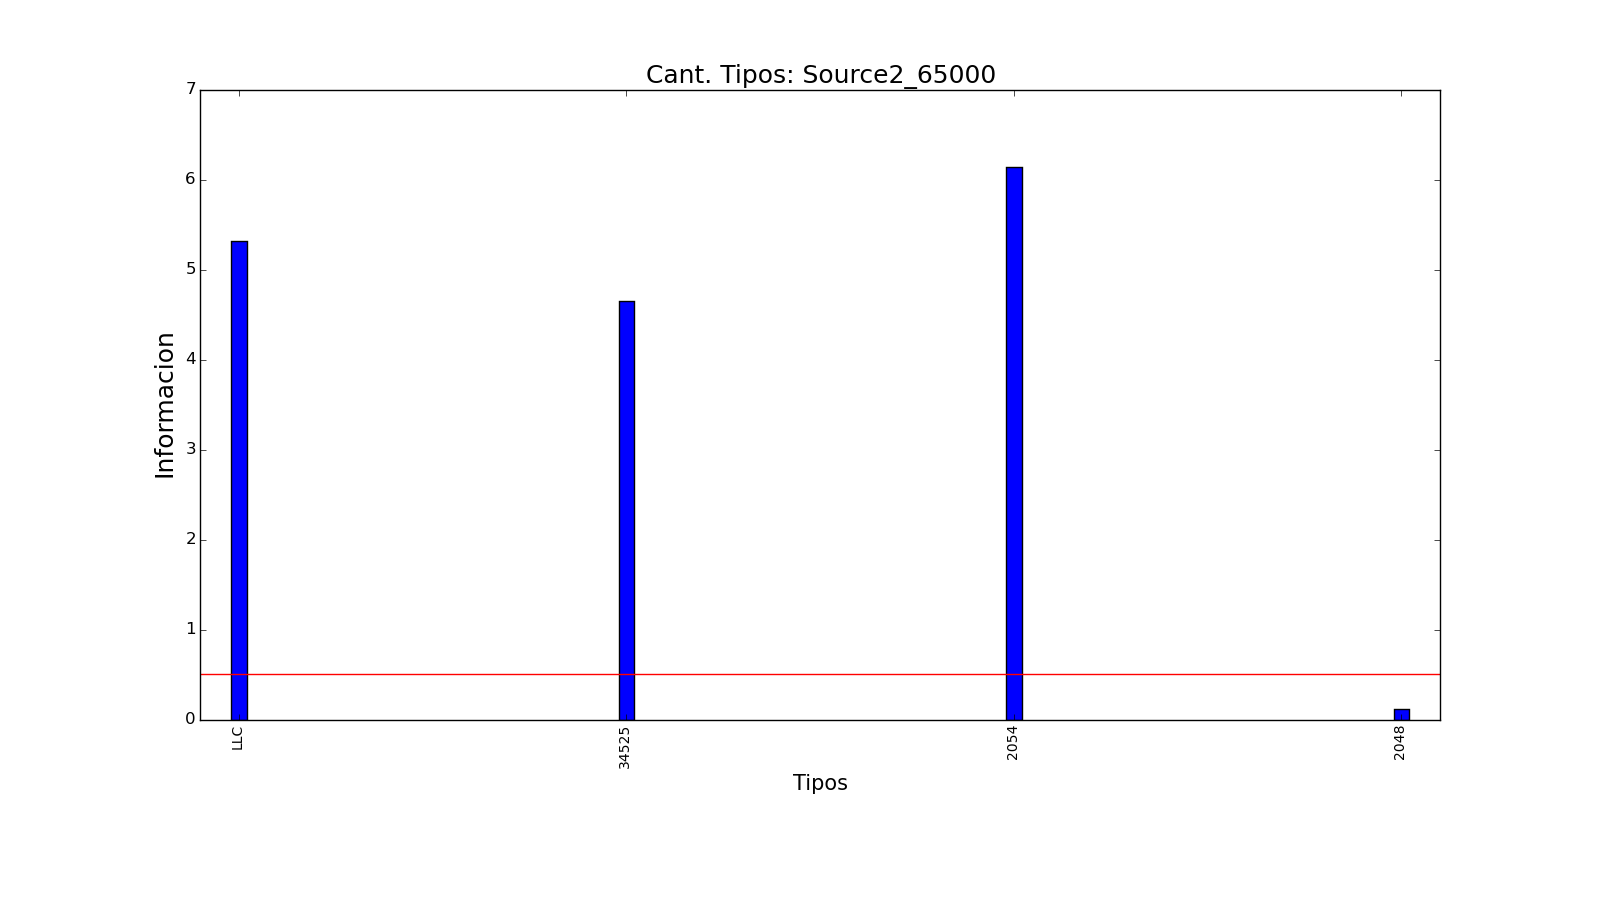
\includegraphics[width=1\textwidth]{../resultados/McDonalds/histogram_types_information.png}
       \caption{Información de los protocolos de los paquetes capturados}
       \label{red-hogarena-types}
\end{figure}

Como podemos observar, de acuerdo a la definición de protocolo distinguido que dimos anteriormente, el protocolo IPv4 sería el único distinguido en esta fuente. Esto resulta razonable, ya que la cantidad de paquetes IPv4 es mucho mayor que la cantidad de paquetes IPv6, LLC y ARP. La información de los paquetes IPv4 es \textbf{0.118172764791}, mientras que la entropía de la fuente es \textbf{0.51288679091}. Se observa claramente como la información es menor a la entropía.

\begin{figure}[H]
       \centering
       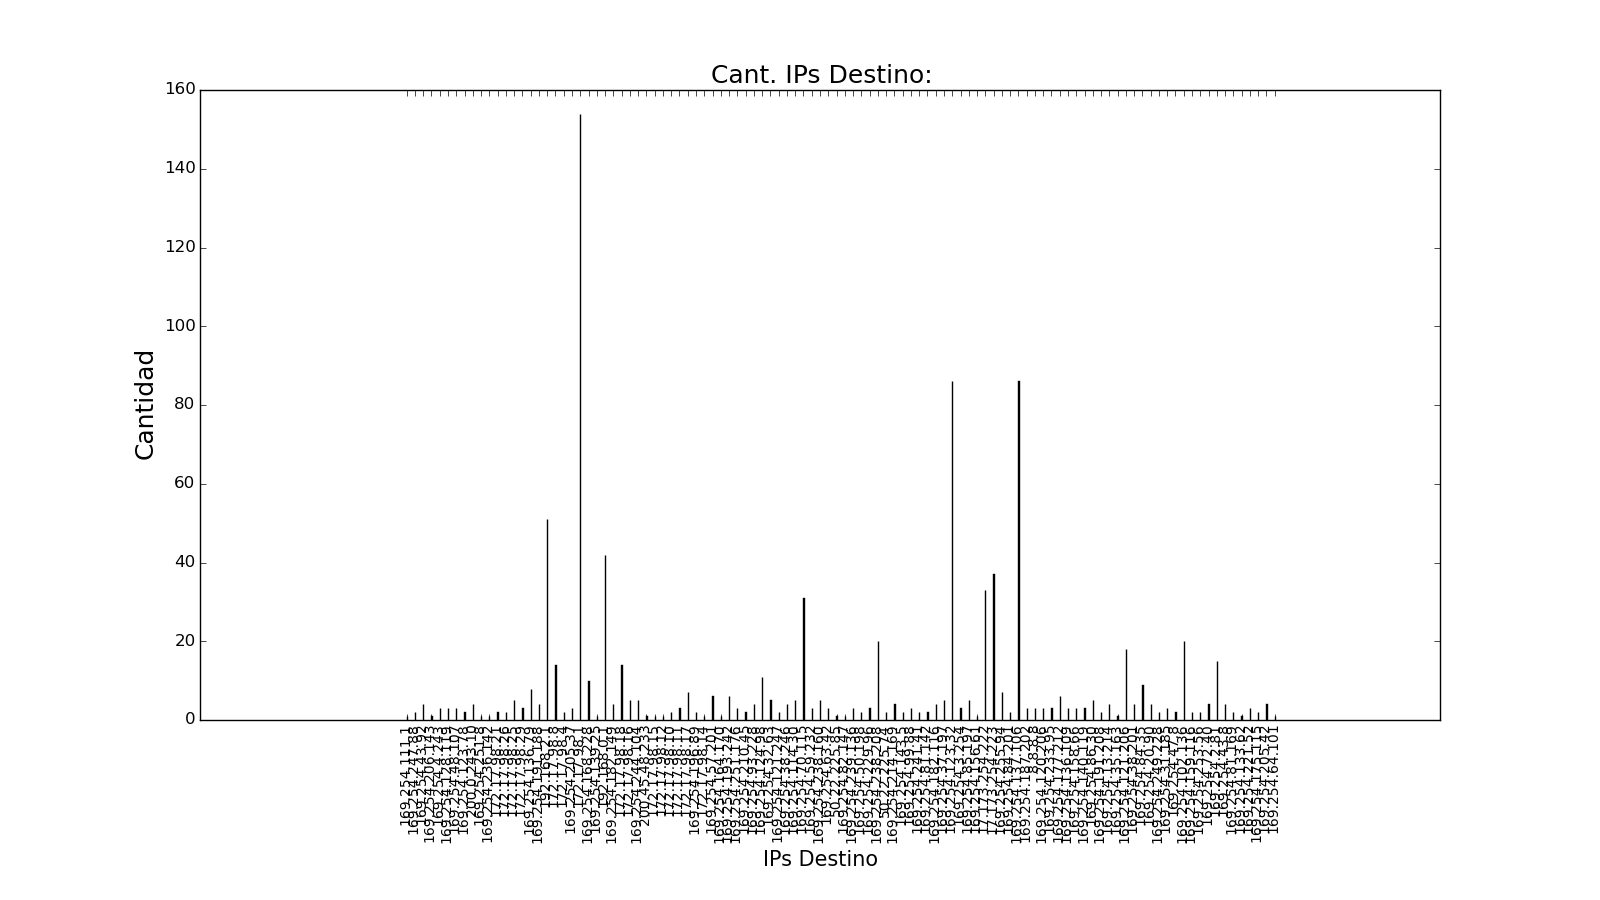
\includegraphics[width=1\textwidth]{../resultados/McDonalds/histogram_dst.png}
       \caption{IPs destino de los paquetes ARP}
       \label{red-hogarena-arp-destination}
\end{figure}

\begin{figure}[H]
       \centering
       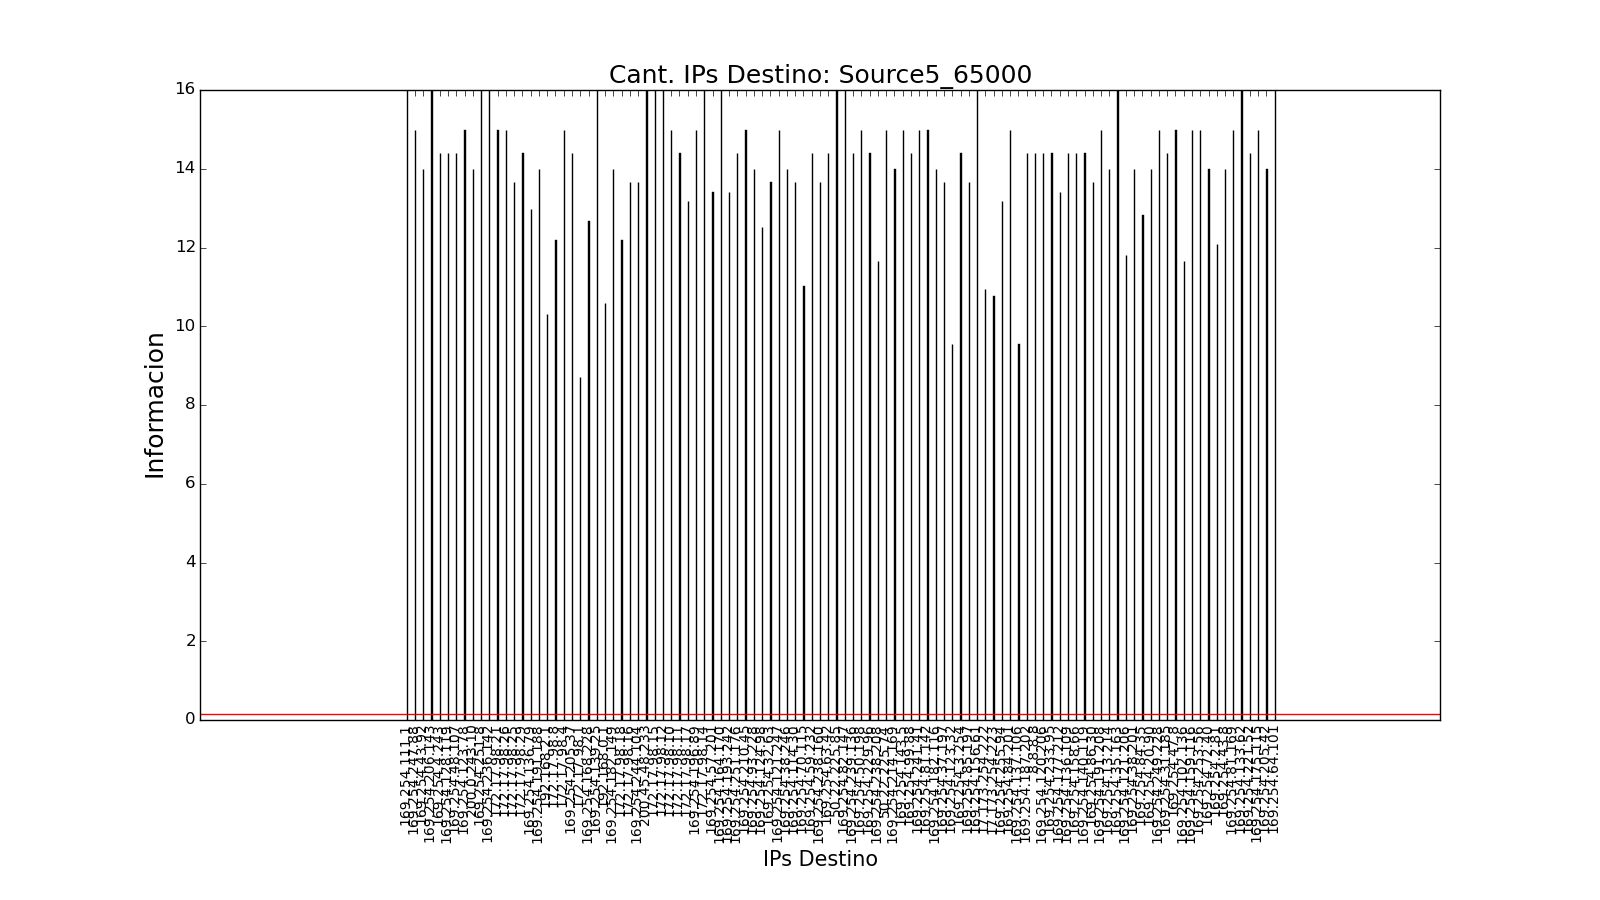
\includegraphics[width=1\textwidth]{../resultados/McDonalds/histogram_dst_information.png}
       \caption{Información de IPs destino de los paquetes ARP}
       \label{red-hogarena-arp-destination-info}
\end{figure}

En este caso el valor de la entropía es de \textbf{5.22269613542}, y se pueden observar ocho IPs que se encuentran debajo de este valor, por lo que consideramos que son nodos distinguidos en la red. Dichas IPs son:
\begin{itemize}
\item IP: \textit{192.168.2.1} con valor de información de \textbf{4.16992500144}
\item IP: \textit{172.17.8.1} con valor de información de \textbf{2.57556380272}
\item IP: \textit{192.168.0.1} con valor de información de \textbf{4.45003292064}
\item IP: \textit{169.254.70.115} con valor de información de \textbf{4.88815403303}
\item IP: \textit{169.254.123.32} con valor de información de \textbf{3.41608558871}
\item IP: \textit{17.173.254.222} con valor de información de \textbf{4.79795622406}
\item IP: \textit{17.173.254.223} con valor de información de \textbf{4.63289697778}
\item IP: \textit{169.254.137.106} con valor de información de \textbf{3.41608558871}
\end{itemize}

Es importante destacar que el nodos con IP:\textit{172.17.8.1} tiene una información mucho menor al resto, por lo que probablemente se trate de un router.

A continuación se muestra el tráfico de la red para poder reconocer con qué dispositivos se condicen los \textbf{nodos distinguidos}

\begin{figure}[H]
       \centering
       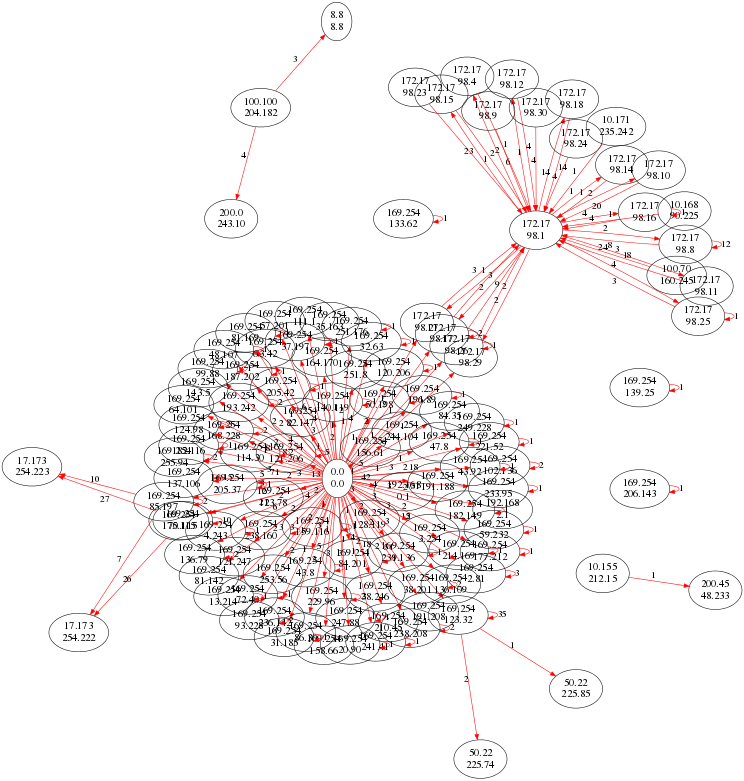
\includegraphics[width=1\textwidth]{../resultados/McDonalds/network.png}
       \caption{Tráfico de paquetes ARP}
       \label{red-hogarena-arp-traffic}
\end{figure}

En este caso se observa que el nodo con IP: \textit{172.17.98.1}, es destino de varios nodos, por lo confirma aun más nuestra hipotesis de que se trate de un router.

Por otro lado es inevitable observar que el nodo con IP: \textit{0.0.0.0} es fuente de una gran cantidad de nodos.

En cuanto al resto de los nodos distinguidos creemos que se tratan de usuarios conectados a internet con una mayor demanda de paquetes que el resto.
